\documentclass[11pt,letterpaper]{article}

% Essential packages
\usepackage{fontspec}
\usepackage[utf8]{inputenc}
\usepackage[T1]{fontenc}
\usepackage{geometry}
\usepackage{amsmath}
\usepackage{amsfonts}
\usepackage{amssymb}
\usepackage{graphicx}
\usepackage{booktabs}
\usepackage{array}
\usepackage{longtable}
\usepackage{multirow}
\usepackage{multicol}
\usepackage{float}
\usepackage{caption}
\usepackage{subcaption}
\usepackage{hyperref}
\usepackage{fancyhdr}
\usepackage{datetime}
\usepackage{enumitem}
\usepackage{listings}
\usepackage{xcolor}
\usepackage{verbatim}
\usepackage{url}
\usepackage{svg}

% Page setup
\geometry{margin=1in}
\setlength{\parindent}{0pt}
\setlength{\parskip}{6pt}

% Header and footer setup
\pagestyle{fancy}
\fancyhf{}
\lhead{Data Science Capstone Journal}
\rhead{\today}
\cfoot{\thepage}
\renewcommand{\headrulewidth}{0.4pt}

% Code listing setup
\lstset{
    basicstyle=\ttfamily\footnotesize,
    backgroundcolor=\color{gray!10},
    frame=single,
    breaklines=true,
    captionpos=b,
    numbers=left,
    numberstyle=\tiny\color{gray},
    keywordstyle=\color{blue},
    commentstyle=\color{green!60!black},
    stringstyle=\color{red}
}

% Custom commands
\newcommand{\journalentry}[2]{
    \section*{Journal Entry - #1}
    \addcontentsline{toc}{section}{Journal Entry - #1}
    \textbf{Date:} #2 \\
    \textbf{Duration:} 10 hours \\
    \rule{\textwidth}{0.5pt}
}

\newcommand{\objective}[1]{
    \subsection*{Objective}
    #1
}

\newcommand{\activities}[1]{
    \subsection*{Activities Completed}
    #1
}

\newcommand{\findings}[1]{
    \subsection*{Key Findings}
    #1
}

\newcommand{\challenges}[1]{
    \subsection*{Challenges Encountered}
    #1
}

\newcommand{\nextSteps}[1]{
    \subsection*{Next Steps}
    #1
}

\newcommand{\reflections}[1]{
    \subsection*{Reflections}
    #1
}

% Title page setup
\newcommand{\workingtitle}{A Physics-Informed Neural Network Approach to Parameter Estimation with User-Driven Exploration and Visualization}
\title{\Large \textbf{DATS 598: Data Science Capstone} \\ 
       \large Journal Entries and Progress Documentation \\
       \vspace{0.5cm}
       \normalsize \textbf{\workingtitle}}
\author{Eric Crisp \\ 
        University of Pennsylvania \\
        \texttt{ecrisp@upenn.edu}}
\date{\today}

\begin{document}

\maketitle
\tableofcontents
\newpage

% ========================================
% SAMPLE JOURNAL ENTRY -- MAIN PROPOSAL
% ========================================

\journalentry{Week 2 - Main Proposal}{\today}

\objective{
Synthesyze the literature review and understand a path forward with respect to the project on PINN, or pivot to alternative project (truth detection).}

\activities{
\begin{itemize}
    \item Whitepaper review of generating simulations from PINN-derived systems of equations deemed too sophisticated for a 12-week project.
    \item Simplification of the proposed PINN project includes removing the equation generation step and focusing on the subset problem space of Parameter Estimation for systems of ODEs. 
    \item Systems of ODEs, or even PDEs if time allows (i.e., heat equation), can be converted from code, to symbolic representations with SymPy, converted to tensors for PyTorch the entire space of linear equations to be considered.
    \item ODEs with algebraic loops need to introduce stale parameters which can be captured symbolically and defined as the i - 1 value (i.e., lagged parameters).
\end{itemize}
}

\findings{
While the full-blown PINN project that was intiated last week was determined to be too expensive and likely unfeasbile, the new task is a simplification and a narrowing of scope. The goal is to now take a system of equations and symbolically convert them to a matrix of coefficients of terms (linear, non-linear differential equations are out of scope), use this system to estimate the parameters via PINN with loss functions tied to fundamental physics and user-defined regularizations. \\

The use case for this kind of application is quite significant. When the Space Shuttle, or any man-rated vehicle is flying, the sensor data stored is significantly less than the data stored on the test stand. So, when  models are made and controllers are developed, the operation in the field relies on much less although critical flight data. Depending on the speed, reliability, and many other factors, a PINN-trained model in the loop could help define concepts such as:
\begin{itemize}
    \item Remaining Product Life
    \item Likelihood of Catostrophic Failure 
    \item Predictions of Unmeasured Data
\end{itemize}

For this project, we will start with a simple model and build to a more complex model that relies on my background in real-time modeling physical systems. The goal is to show how a trained model can predict, or connect the dots when information is missing, if the parameters estimated are sound. For example, imagine a web app with a diagram of a rocket engine. You have 15 sensors available to "include" in the training, but when flying, you must choose only 5. The predictions (i.e., likelihood of failure, or of the sensors not selected) can vary wildly depending on which 5 are selected, the loss functions included in training, and other factors. This can be visualized by simulation accuracy in the time domain, as well as an overall accuracy in the steady state domain.

}

\challenges{
\begin{itemize}
    \item Leverage aerospace background and create two systems of ODEs that can be used for testing parameter estimation: 
    \begin{itemize}
        \item trial and experimentation (fluid flow in a pipe with a chemical reaction)
        \item full-scale implementation of application (i.e., rocket engine system)
    \end{itemize}
    \item Create the generic systems of equations, convert them to tensors with SymPy, ensure algebraic loops are broken, and apply automatic differentiation.
    \item Create underlying pipeline from Python model to deployed (i.e., inference) on web app with parameter selection and vizuations.
\end{itemize}
}

% ========================================
% SAMPLE JOURNAL ENTRY -- SECONDARY PROPOSAL
% ========================================

\newpage
\journalentry{Week 2 - Secondary Proposal}{\today}

\objective{
AI text generation can be incorrect in multiple ways. This project considers a simple, toy process for detecting whether the facts presented in a prompt (i.e., generated response) are likely true or not.
}

\activities{
\begin{itemize}
    \item The FEVER dataset \footnote{\href{https://fever.ai/dataset/fever.html}{https://fever.ai/dataset/fever.html} is a dataset commonly used for training truth detection.} contains a large number of samples scraped from Wikipedia that are considered to be "true" along with modifications to them that are considered "false".
    \item This process of truth detection would include significant semantic analysis, natrual language processing techniques, as well as data wrangling. 
    \item Ideally, this would be turned into a web-app where the user could type in a statement, or question, and the result would be a likelihood that it is true.
    \item Extensions of this could be tied into responses from LLM to give the user a degree of confidence external to the text-generating tool itself.
\end{itemize}
}

\findings{
The project timeline for this would be feasible as many of the tools are open source, the beginning dataset is well-known, and there is room to expand by including things like RAG and web scraping instead of relying on the information in FEVER.
}

\challenges{
\begin{itemize}
    \item NLP algorithms for understanding what is the fact that under consideration.
    \item Understanding what defines "trustworthy" relative to web data (i.e., what is "truth" and at what point when does X\% "truth" becomes fake, or false).
    \item Data wrangling and pipeline process, more than just FEVER, incorporating a database consisting of cleaned, preprocessed web data.
\end{itemize}
}

\nextSteps{
\begin{enumerate}
    \item Create clean-cut skeleton of the process, tooling, dataset, and libraries needed with timelines associated to implement neccesary applications, or extensions.
\end{enumerate}
}

\reflections{
As the scope of this project is being honed, the two viable paths that remain are an NLP, web scraping and data wrangling project and a project centered around deep neural networks that overlaps with differential equations. Both projects involve heavy, yet distinctly different, aspects of data science and machine learning. The main takeaway of the NLP project

\begin{table}[h!]
\centering
\begin{tabular}{|>{\centering\arraybackslash}p{3.5cm}|
                >{\centering\arraybackslash}p{5cm}|
                >{\centering\arraybackslash}p{5cm}|}
\hline
\textbf{Aspect} & \textbf{PINN Parameter Estimation} & \textbf{NLP Truth Detection} \\
\hline
Model(s) & PINN & Physics-Informed NN \\
Training Data & Synthetic (simulation) & FEVER, web-scraping, RAG \\
Loss Function & Physics-based, MSE & MSE, Logistic Regression \\
Tooling and Overhead & Significant, excluding the additional web app interface & Minimal, except web app \\
Tech Stack & Python, FastAPI, PyTorch, Pandas & Python, JavaScript (Node, React)\\
\hline
\end{tabular}
\caption{Comparison of PINN Parameter Estimation and NLP-based Truth Detection}
\end{table}


}

% ========================================
% APPENDICES (if needed)
% ========================================

% % symbols for directory modeling: ├  └  │  ─  ┬  ┼  ═
\newpage
\appendix
\section{Systems of Equations for PINN Implementation}
\subsection*{A. Simple Case: Mass Spring Damper System}

Generically, this is a well understood system and includes the states and learned parameters.

\begin{equation}
\begin{aligned}
x_1 &= x(t), \quad x_2 = \dot{x}(t) \\
\dot{x}_1 &= x_2 \\
\dot{x}_2 &= \frac{1}{m} \left( -c x_2 - k x_1 + F(t) \right)
\end{aligned}
\end{equation}

\begin{figure}[htbp]
  \centering
  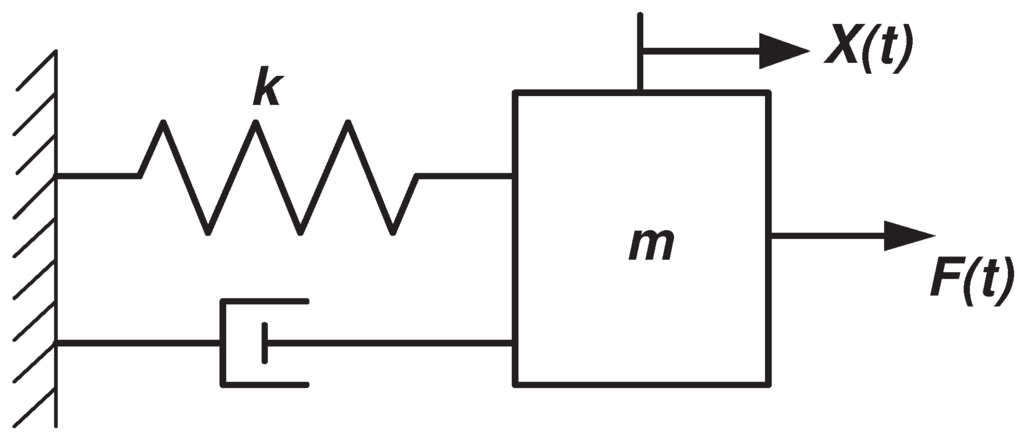
\includegraphics[width=0.25\textwidth]{../../documents/images/mass-spring-damper-system.png}
  \caption{Simple Mass-Spring-Damper System}
  \label{fig:mass-spring-damper-diagram}
\end{figure}

This sets the parameters to be estimated as \\
$$\theta = \{ m, c, k \}$$ 

\subsection*{B. Complex Case: Liquid Rocket Engine Systeme Model}

The RS-25, or Space Shuttle Main Engine, is a well known rocket engine that is relatively simple to simulate. A system of equations can be created to model the components. There are N parameters and M states where a parameter can be learned (i.e., line resistances, discharge coefficients, etc.) and a state is defined as a variable that dictates a state within the engine (i.e., chamber pressure, turbopump shaft speed, etc.). The system of equations is produced below and will be converted into matrix format after simulations show that numeric stability as the timeseries data here is used as samples for PINN training.

PCA and other dimensional reduction methods can, and should be, used to determine which sensors (states) are most critical to the sytem.

\begin{align}
f_1(x, y) &= 0 \\
f_2(x, y) &= 0
\end{align}

\begin{figure}[htbp]
  \centering
  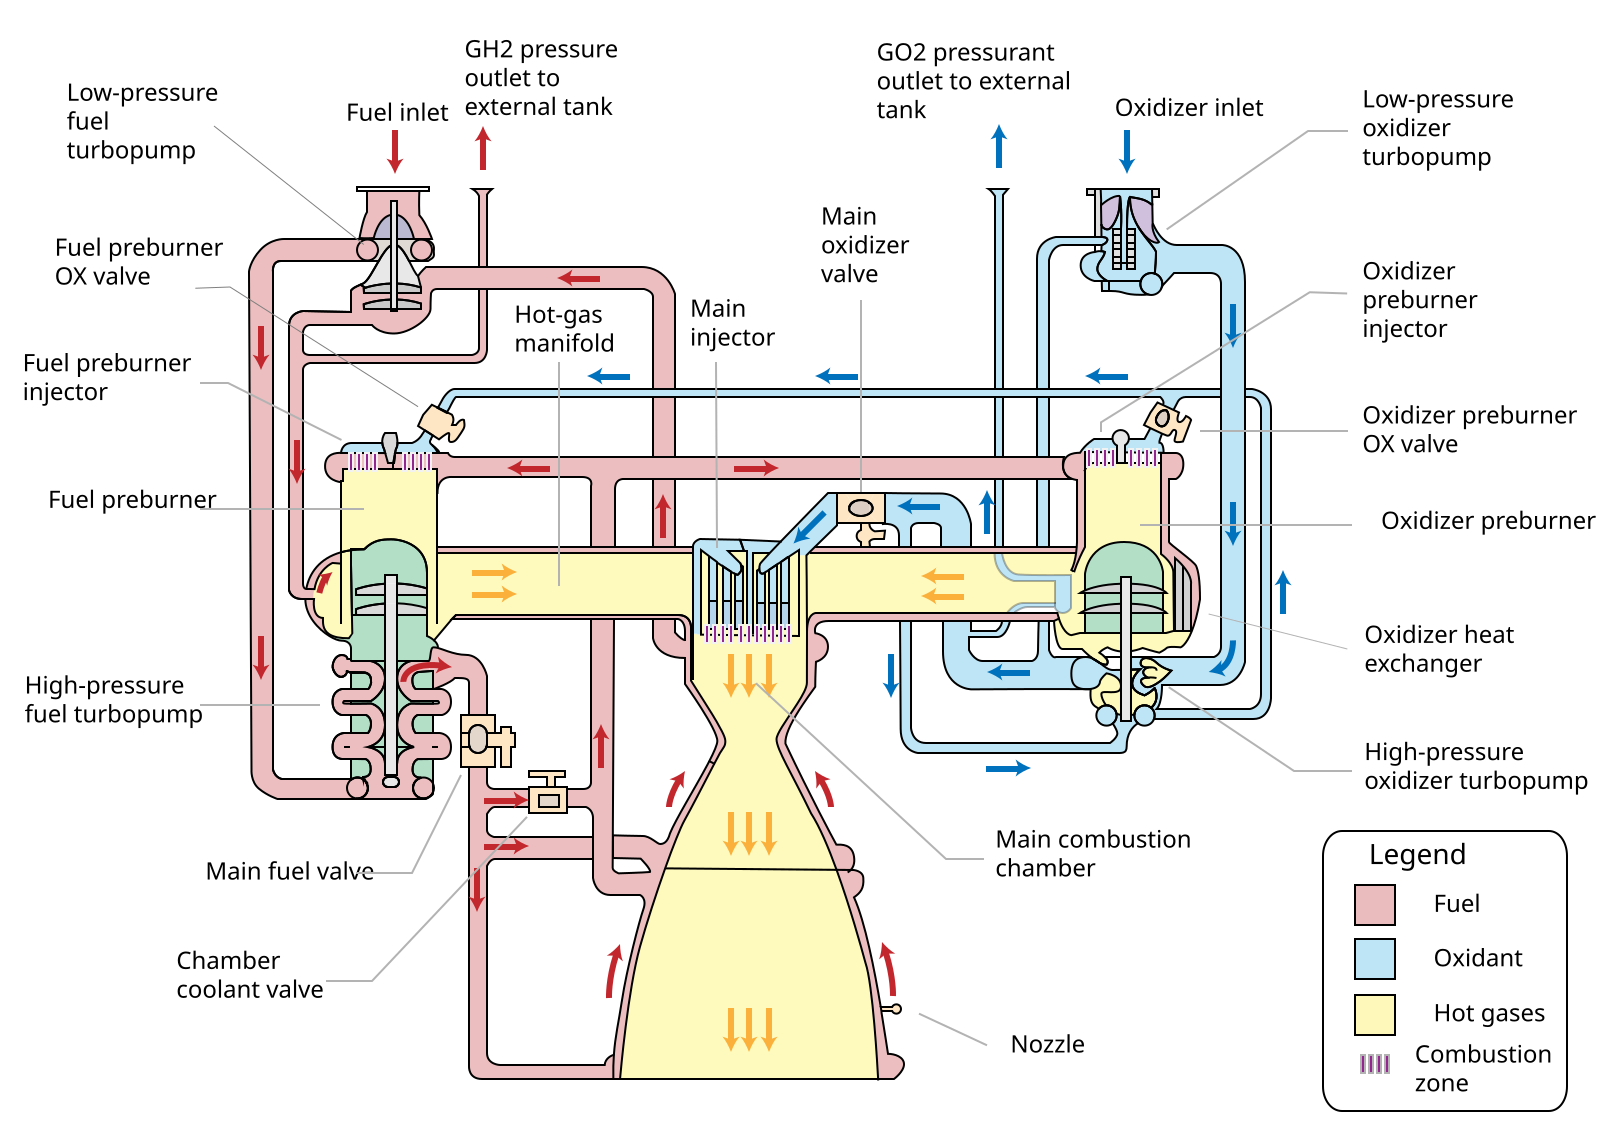
\includegraphics[width=0.5\textwidth]{../../documents/images/SSME_engine_schematic}
  \caption{Space Shuttle Main Engine (RS-25) Engine Diagram}
  \label{fig:SSME_engine_diagram}
\end{figure}

\end{document}